\section{Denise}\label{sec:algorithm}

Mathematically, PCA is the eigenvalue decomposition of correlation-, respectively covariance-matrices, obtained from data. Such matrices $M$ are always positive semi-definite. Therefore, they are diagonalizable $M = \tilde{U}\Lambda \tilde{U}^T$ with orthogonal matrix $U$ and diagonal matrix $\Lambda = \diag{\lambda_1,\dots,\lambda_n}$ having the eigenvalues of $M$ on the diagonal. The columns of $U$ are the eigenvectors of $M$. We can absorb the diagonal matrix $\Lambda$ in $\tilde{U}$ and $\tilde{U}^T$ by multiplying each column of $U$ with the square root of the corresponding eigenvalue $U_{i,j} = \tilde{U}_{i,j} \sqrt{\lambda_j}$ for all $i,j$, or equivalently $U = \sqrt{\Lambda}\tilde{U}$ with $\sqrt{\Lambda} = \diag{\sqrt{\lambda_1},\dots,\sqrt{\lambda{n}}}$. This results in the decomposition $M = \tilde{U}\sqrt{\Lambda} \sqrt{\Lambda} \tilde{U}^T = UU^T$. Note that usually $U$ is not orthogonal, anymore. On the other hand, from a given decomposition $M = UU^T$ of a positive semi-definite $M$ we can always obtain the eigenvalues $\lambda_i$ of $M$ as the square of the 2-norm of the columns of $U$ and by this obtain the ordinary eigenvalue decomposition $M = \tilde{U}\Lambda\tilde{U}^T$ with $\tilde{U}_{i,j} = U_{i,j}/\sqrt{\lambda_j}$.

The above, obviously, only works for square-matrices which are additionally positive semi-definite. However, for \textit{any} matrix $M$, given for example a $n\times m$ data-matrix of $m$ observations of $n$ features, we can calculate the singular value decomposition (SVD) $M = \tilde{U} (\Lambda, 0) \tilde{V}^T$ (here, we assume $m\geq n$; the other case is very similar). $U$ is a orthogonal $n\times n$-matrix, $V$ is an orthogonal $m\times m$ matrix and $(\Lambda, 0)$ is a diagonal rectangular $n\times m$ matrix with $\Lambda = \diag{\lambda_1,\dots,\lambda_n}$ in the first $n$ columns and $0$ everywhere else. The columns of $\tilde{U},\tilde{V}$ are the left, respectively right, singular vectors of $M$ and $\lambda_1,\dots,\lambda_n$ are its singular values. As above in the case of the eigenvalue decomposition, the SVD of $M$ is equivalent to the decomposition $M = UV^T$ with $n\times n$-matrix $U = \tilde{U}\sqrt{\Lambda}$ and $n\times m$-matrix $V^T = (\sqrt{\Lambda}, 0) \tilde{V}^T$. Note that the SVD is not unique, but is always exists. Moreover, the eigenvalue decomposition is a special case of the more general SVD which, if applicable, is in fact unique up to permuting the eigenvectors in $U$.

In the following we describe an approach based on neural networks, to obtain the eigenvalue decomposition (i.e. PCA) of positive semi-definite matrices, respectively the SVD of general matrices. Moreover, this decomposition should be of low rank $k<n$, meaning that we want to restrict to an approximate decomposition $M \approx UV^T$ with $n\times k$-matrix $U$ and $m\times k$-matrix $V$. In this approximation, the columns of $U,V$ approximate the $k$ left, respectively right, singular vectors corresponding to the $k$ largest singular values of $M$. If the remaining $n-k$ singular values are indeed very small in comparison with those, then the rank-$k$ decomposition is justified an yields a valid approximation. We tackle the rank-$k$ decomposition $M \approx UV^T$ by learning the map from $M \mapsto U,V$ by a neural network trained on a suitable synthetic dataset $(M_i,(U_i,V_i))_i$ of such matrices, as described in detail subsequently. 



\subsection{Eigenvalue decomposition of positive semi-definite matrices (covariance matrices)}
 
We consider $\mathbb{S}_n \subseteq \mathbb{R}^{n \times n}$ to be the set of $n$-by-$n$ symmetric matrices and $P_n\subseteq \mathbb{S}_n$ to be the subset of positive semi-definite matrices and $P_{k,n} \subseteq P_n$ the subset of matrices with rank at most $k$. As the input of our deep neuronal network we consider a Matrix $M = [M_{i,j}]_{i,j} \in P_n$. $M$ is to be decomposed as a sum $M = L + S$ where $L = [L_{i,j}]_{i,j} \in P_{k,n}$ is of rank at most $k$ and a sparse matrix $S = [S_{i,j}]_{i,j} \in P_n$. Since $L$ is assumed to be symmetric, by the Cholesky decomposition, we can represent it as $L=UU^T$, where $U = [U_{i,j}]_{i,j} \in \mathbb{R}^{n \times k}$. Therefore $M$ can be expressed as $M = UU^T + S$.

\paragraph{Loss function}
We input $M$ in the neural network, which should faithfully output the low rank matrix $U$. Hence, we want to minimize the difference between $M$ and $UU^T$, which is equal to $S$. A convenient choice of loss-function for the considered neural network is, therefore, given by the $\ell_1$-matrix-norm of $S$
\[
\Vert UU^T - M \Vert_{\ell_1} = \Vert S \Vert_{\ell_1}
\]
The $\ell_1$-norm is a common choice to guarantee sparsity of $S$.

\paragraph{Architecture}
As the matrix M is symmetric, we can reduce the input from $n^2$ to $n(n + 1)/2$ by taking the triangular lower matrix of $M$. The lower matrix is then transformed into a vector using the operator h:
\[
h: S^n \to \mathbb{R}^{n(n+1)/2}, \, M \mapsto (M_{1,1},M_{2,1},M_{2,2},\dots,M_{n,1},\dots,M_{n,n})^T
\]
Similarly we convert the output vector of the neural network into a matrix with the operator g defined as
\[
g : \mathbb{R}^{nk} \to \mathbb{R}^{n \times k}, \, X \mapsto \begin{pmatrix} X_1 & \cdots & X_k \\ \vdots & & \vdots \\ X_{(n-1)k + 1} & \cdots& X_{(n-1)k+k}\end{pmatrix}
\]
Besides the output layer, our multi-layer feed-forward neural network $\mathcal{N}: \mathbb{R}^{n(n+1)/2} \to \mathbb{R}^{nk} $ has three hidden dense layers, each exhibiting ReLU-activation function and $n/2$ nodes. Using $h$ and $g$ the matrix $U$ is the output of the neural network $U = g(\mathcal{N}(h(M)))$ and we  get the desired matrix $L=\rho(\mathcal{N}(h(M)))$ for
\[
\rho : \mathbb{R}^{rd} \to P_{r,d}, X \mapsto g(X)g(X)^T
\]


\paragraph{Generation of training data}
For the training of Denise a synthetic dataset, consisting of randomly generated matrices with appropriate decomposition properties, is created. In detail, we construct a sample of positive semidefinite $n$-by-$n$ matrices $M$ that can be decomposed as
\[
 M = L_0 + S_0
\]
where $L_0$ is a known matrix of rank $k_0 \leq n$ and $S_0$ a known matrix with a given sparsity $s_0$. Here, we undestand a \textit{sparse matrix} as a matrix containing a lot of zeros and define the ratio between the number of zero-valued entries and the total number of entries as its \textit{sparsity}. In the process of data generation, we follow a reverse approach by constructing first the matrices $L_0$ and $S_0$ with the required properties and merge it together to a matrix $M$ which has by definition the desired decomposition.

For the construction of the low-rank matrix $L_0$, we collect $nk_0$ samples of independent standard normal random variables into an $n$-by-$k_0$ matrix $U$ and set $L_0 = UU^T$. This construction scheme guarantees symmetry and positive semidefiniteness of $L_0$ as well as rank $L_0 \leq k_0$. To construct the symmetric positive semidefinite sparse matrix $S_0$, we first take a sample of a uniformly random pair $(i,j)$ with $1 \leq i < j \leq n$ that defines four non-zero entries of an $n$-by-$n$ matrix $\tilde{S_0}$. The off-diagonal elements $(i,j)$ and $(j,i)$ are set to value $b$ as the realization of a uniformly random variable in $[-1,1]$ while the diagonal elements $(i,i)$ and $(j,j)$ are set to value $a$ as the realization of a uniformly random variable in $[\vert b \vert,1]$. Due to its construction $\tilde{S_0}$ is positive semidefinite. Finally, we receive the matrix $S_0$ by summing the realizations $\tilde{S_0}^{(i,j)}$ over the pairs $(i,j)$ until the pursued sparsity is reached. According to the described approach, we define a class \textit{SyntheticMatrixSet} which is, by its methods, able to create a randomly generated matrix $M$ together with $L_0$ and $S_0$ as both parts of its decomposition  $M = L_0 + S_0$ based on the userspecified arguments: dimension $n$, rank $k_0$ and sparsity $s_0$. This class enables the generation of highly extensive datasets for various training purposes.


\subsection{Singular value decomposition of arbitrary matrices (data matrices)}

In the preceding section, we aimed at learning the mapping $M\mapsto U$ for the decomposition $M = UU^T$ by means of a neural network through minimizing the loss $\Vert UU^T - M \Vert_{\ell_1}$. To obtain the low rank-$k$ ($k<n$) SVD $M = UV^T$ of a arbitrary $n\times m$-matrix $M$ into $n\times k$-matrix $U$ and $m\times k$-matrix $V$ we proceed in a similar fashion. However, in this case we train two neural networks $\mathcal{N}_U$ and $\mathcal{N}_V$, one for each mapping $M\mapsto U, M\mapsto V$, by minimizing the loss
\[
\Vert UV^T - M \Vert_{\ell_1} \,.
\]
The $\ell_1$ norm results is used, as above, to force sparsity of the difference $S = UV^T -M$. Obviously, the loss function depends on the predictions of both neural networks. After training, the prediction of the combined network for a given input $M_\text{truth}$ is given by
\[
M_\text{pred} = \mathcal{N}_U(M_\text{truth})\mathcal{N}_V(M_\text{truth})^T ,.
\]
Training the networks parallel at the same time is computationally expensive for large matrices $M$. Therefore, we propose to train both networks in an alternating manner, through successively optimizing the weights of one network by keeping the weights of the others fixed, and vice versa. This procedure must be repeated for several iterations to obtain a reasonable prediction accuracy.

\paragraph{Architecture}
The architectures of both networks $\mathcal{N}_U,\mathcal{N}_V$ are chosen similar to the network $\mathcal{N}$ of the previous section. We choose three hidden dense layers, densely connected to the output layer of dimension $n\times k$, respectively $m\times k$. The first and third hidden layer have $n*m$ nodes, each, while the second layer has $n*m/2$ nodes. Compared to the decomposition of positive semi-definite matrices above, we are not allow to restrict to the lower triangular part of $M$ as input for the network, since $M$ is not necessary symmetric (not even quadratic).


\paragraph{Generation of training data}

The training data is generated similar to above. However, here we generate $U$ and $V$ by sampling their components from independent standard normal distributions. The sparse matrix $S$, representing possible corruptions of the data, is at first initialized as $n\times m$-matrix with zero entries everywhere. Subsequently we uniformly choose entries $(i,j)$ and filling these with random real number following a uniform distribution on $[-1,1]$. This es repeated until the fraction of non-zero entries $r/n*m >0.05$ ($r$ is the number of non-zero entries) arrives at a value larger then a pre-defined threshold (we choose here 0.05). From $U,V,S$ we generate the matrix $M = UV^T + S$, which will be given to the neural networks as training data. Differently then above, we do not need a positive semi-definite $M$ here, hence we do not need to use a special generation procedure to enforce positivity of $S$.

\paragraph{Testing}
For a fist impression of the performance of the neural network SVD, we test the trained two-fold network $(\mathcal{N}_U,\mathcal{N}_V)$ on synthetic test-matrices generated by the same procedure as the training data. For testing, we choose $5\times 4$-matrices and aim at a rank-$2$ decomposition $M = UV^T$ in $5\times 2$-matrix $U$ and $4\times 2$-matrix V. We train the network on a training set of size $100000$ (from which we split of $0.2$ as validation dataset) for $20$ iterations, where in each iteration each network part is trained for 5 epochs. This results in a total number of 200 epochs. We do this with batch-size $64$. The progression of the loss-function and a metric, measuring the sparsity of $S = M - UV^T$, during training is depicted in Fig. \ref{fig:SVD_training_loss_sparsity} for, both, the training and validation data.
\begin{figure}
\centering
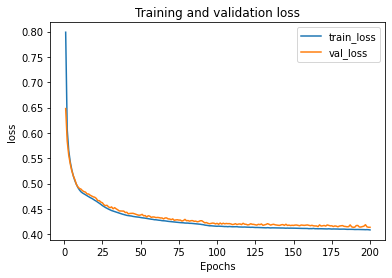
\includegraphics[width=0.48\textwidth]{fig/loss_SVD_[5,4]_k2.png}
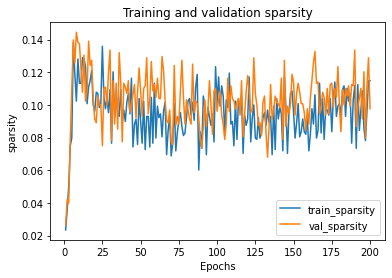
\includegraphics[width=0.48\textwidth]{fig/sparsity_SVD_[5,4]_k2.png}
\caption{Evolution of loss and sparsity-metric on the training and validation data during training over $20\times 5\times 2$ epochs (see main text for explanation)}
\label{fig:SVD_training_loss_sparsity}
\end{figure}
The trained neural network is then tested on three random test matrices $M$, generated as described above. The results are shown in Fig. \ref{fig:SVD_testMLS}. The neural network prediction $L = \mathcal{N}_U(M_\text{truth})\mathcal{N}_V(M_\text{truth})^T$ are quite accurate approximations of actual input matrices $M_\text{truth}$, as one can observed from the matrix-plots. Also the matrices $S = M -L$ are relatively sparse.
\begin{figure}
	\centering
	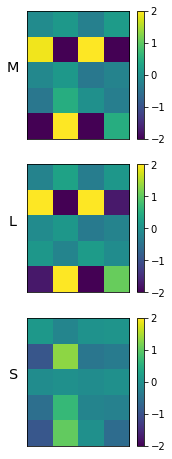
\includegraphics[width=0.25\textwidth]{fig/SVD_testMLS1_[5,4]_k2.png}
	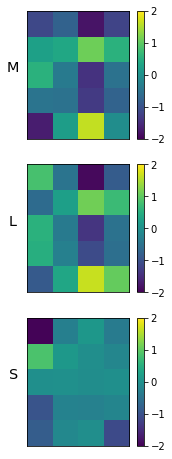
\includegraphics[width=0.25\textwidth]{fig/SVD_testMLS2_[5,4]_k2.png}
	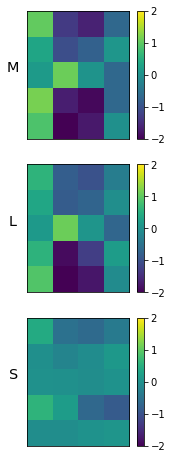
\includegraphics[width=0.25\textwidth]{fig/SVD_testMLS3_[5,4]_k2.png}
	\caption{Testing the $M = L + S$ decomposition (with $L=UV^T$) for $U,V$ calculated from the trained combined neural network $(\mathcal{N}_U,\mathcal{N}_V)$.}
	\label{fig:SVD_testMLS}
\end{figure}


This first test, shows the general capabilities of the presented neural network approach to calculate the robust SVD of arbitrary matrices $M$. However, in the following, we will mostly restrict to the simpler robust low-rank decomposition $M = UU^T$ of a positive semi-definite input matrix $M$. This is a very common situation in practice and of great relevance, for example in the PCA of correlation matrices.


